\chapter{移动平台设计和制造}
\label{cha:Platform}

% \section{现有平台对比}

% 从各类文献和实验平台中总结出各种移动平台的技术参数见表~\ref{tab:Comparison},


% % \begin{figure}[htbp]
% %     \centering
% %     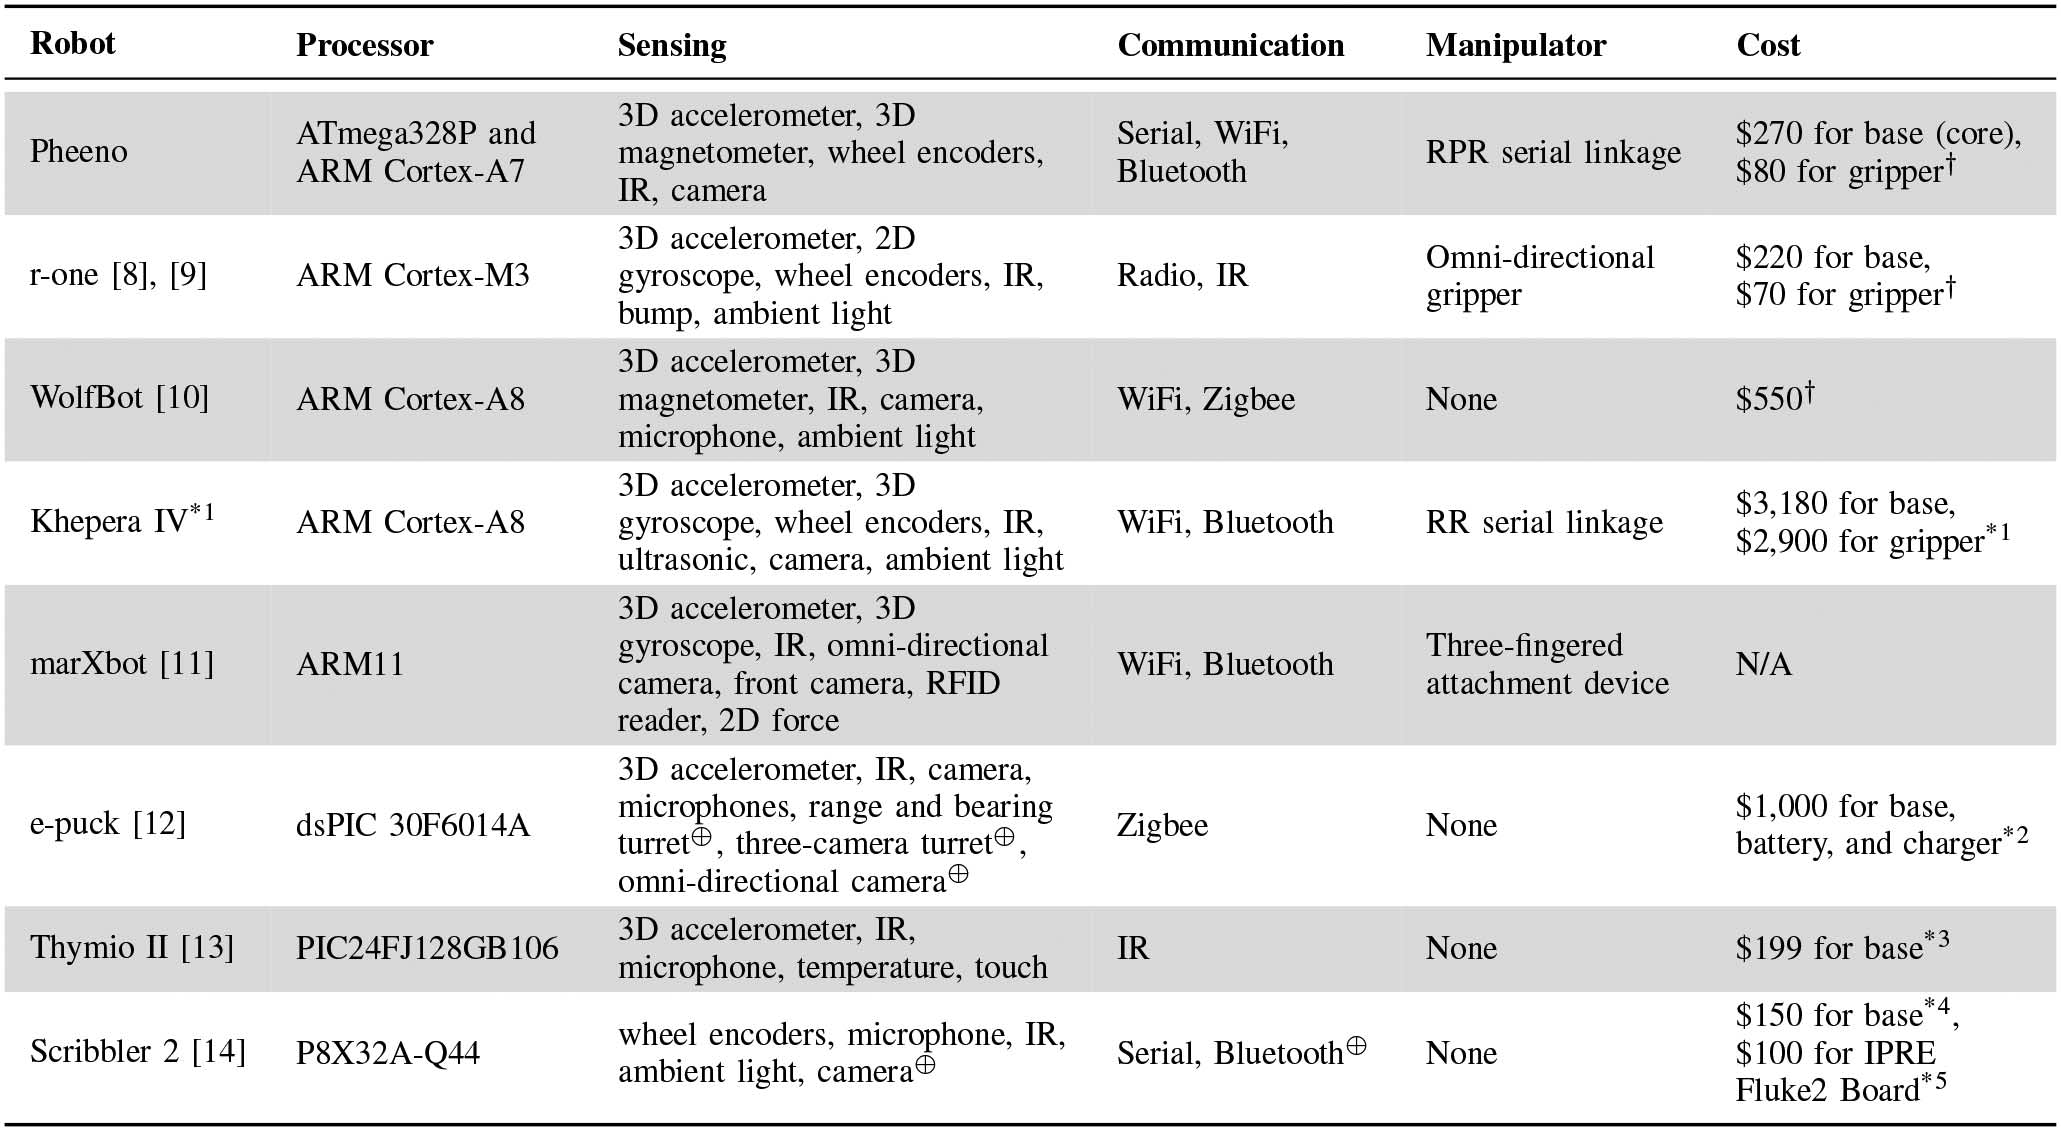
\includegraphics[height=8cm]{Pheeno.jpg}
% %     \caption{COMPARISON OF CURRENTLY AVAILABLE MULTI-ROBOT PLATFORMS\cite{wilson2016pheeno}}
% %     \label{fig:Pheeno}
% % \end{figure}

% % Please add the following required packages to your document preamble:
% % \usepackage[table,xcdraw]{xcolor}
% % If you use beamer only pass "xcolor=table" option, i.e. \documentclass[xcolor=table]{beamer}
% % \usepackage{lscape}
% \begin{landscape}
%     \begin{table}[htbp]
%     \centering
%     \begin{tabular}{lllllll}
%     \hline
%     Name        & Processor                                                                  & Sensing                                                                                                                & Comm.                                                                     & Imaging                                                                              & Cost                 \\ \hline
%     \rowcolor[HTML]{EFEFEF} 
%     R-One       & \begin{tabular}[c]{@{}l@{}}ARM Cortex-M3, \\ 50 MHz, 64KB RAM\end{tabular} & \begin{tabular}[c]{@{}l@{}}Accelerometer,\\ Gyroscope, Bump, \\ IR, Ambient Light\end{tabular}                         & \begin{tabular}[c]{@{}l@{}}Radio (2 Mbps), \\ IR (1.25 Kbps)\end{tabular} & None                                                                                 & \$220 (Parts)        \\
%     E-puck      & \begin{tabular}[c]{@{}l@{}}dsPIC 30F6014A, \\ 64MHz, 8KB RAM\end{tabular}  & \begin{tabular}[c]{@{}l@{}}IR, Accelerometer, \\ Microphone, Camera\end{tabular}                                       & Serial, Bluetooth, IR                                                     & \begin{tabular}[c]{@{}l@{}}40x40 pixels @ 4 FPS. \\ External processing\end{tabular} & \$340 (Parts)        \\
%     \rowcolor[HTML]{EFEFEF} 
%     MarXBot     & \begin{tabular}[c]{@{}l@{}}ARM11, 533 MHz, \\ 128MB RAM\end{tabular}       & \begin{tabular}[c]{@{}l@{}}Camera,\\ Accelerometer, \\ Gyroscope, RFID, \\ 2D Force, \\ Microphone\end{tabular}        & WiFi, Bluetooth                                                           & \begin{tabular}[c]{@{}l@{}}Up to 2048x1536\\ pixel s @ 12 FPS\end{tabular}           & N/A                  \\
%     Khepera III & \begin{tabular}[c]{@{}l@{}}XScale, 600MHz, \\ 128MB RAM\end{tabular}       & \begin{tabular}[c]{@{}l@{}}IR, Ambient Light,\\ Ultrasonic, Camera\end{tabular}                                        & WiFi, Bluetooth                                                           & 640x480 pixels @ 15 FPS                                                              & \textgreater{}\$2000 \\
%     \rowcolor[HTML]{EFEFEF} 
%     CITRIC      & \begin{tabular}[c]{@{}l@{}}XScale, 624 MHz, \\ 64MB RAM\end{tabular}       & \begin{tabular}[c]{@{}l@{}}Camera, \\ Microphone\end{tabular}                                                          & Zigbee                                                                    & 1280x1024 pixels @ 15FPS                                                             & \$600                \\
%     WolfBot     & \begin{tabular}[c]{@{}l@{}}ARM Cortex-A8, 1GHz, \\ 512MB RAM\end{tabular}  & \begin{tabular}[c]{@{}l@{}}IR, Camera, \\ Microphone, \\ Ambient Light, \\ Accelerometer, \\ Magnetometer\end{tabular} & WiFi, Zigbee                                                              & Up to 1280x720 pixels @ 50 FPS                                                       & \$550 (Parts)       
%     \end{tabular}
%     \caption{Mobile Sensing Platform Comparison\cite{betthauser2014wolfbot}}
%     \label{tab:Comparison}
%     \end{table}
% \end{landscape}

\section{平台设计思路}
形式:

每个小车为一个数据点,在1-3维坐标系内动态运动(如果和ShapeBots\cite{suzuki2019shapebots}一样具备升降平台或者和SwarmOS一样具备可变色LED点阵则可以进行三维变量显示)

也可以每个小车作为一个通信节点(在电力市场的应用场景下是一个机组节点),用屏幕/位置/RGB颜色/高度直观的显示迭代的过程。

即插即用的实现:放入/取出小车,新的迭代随即开始。

\section{仿真}

Swarm仿真参考ShapeBots\cite{suzuki2019shapebots}的仿真方法\footnote{\href{https://ryosuzuki.github.io/shapebots-simulator/}{https://ryosuzuki.github.io/shapebots-simulator/}},使用Javascript在网页端编写了相应的仿真程序,进行指定数量的集群小车对于SVG格式图片的渲染和给定数据折线图或条形图的可视化绘制。

\section{定位方法}

% % 如果直接插入一页PDF用
% % 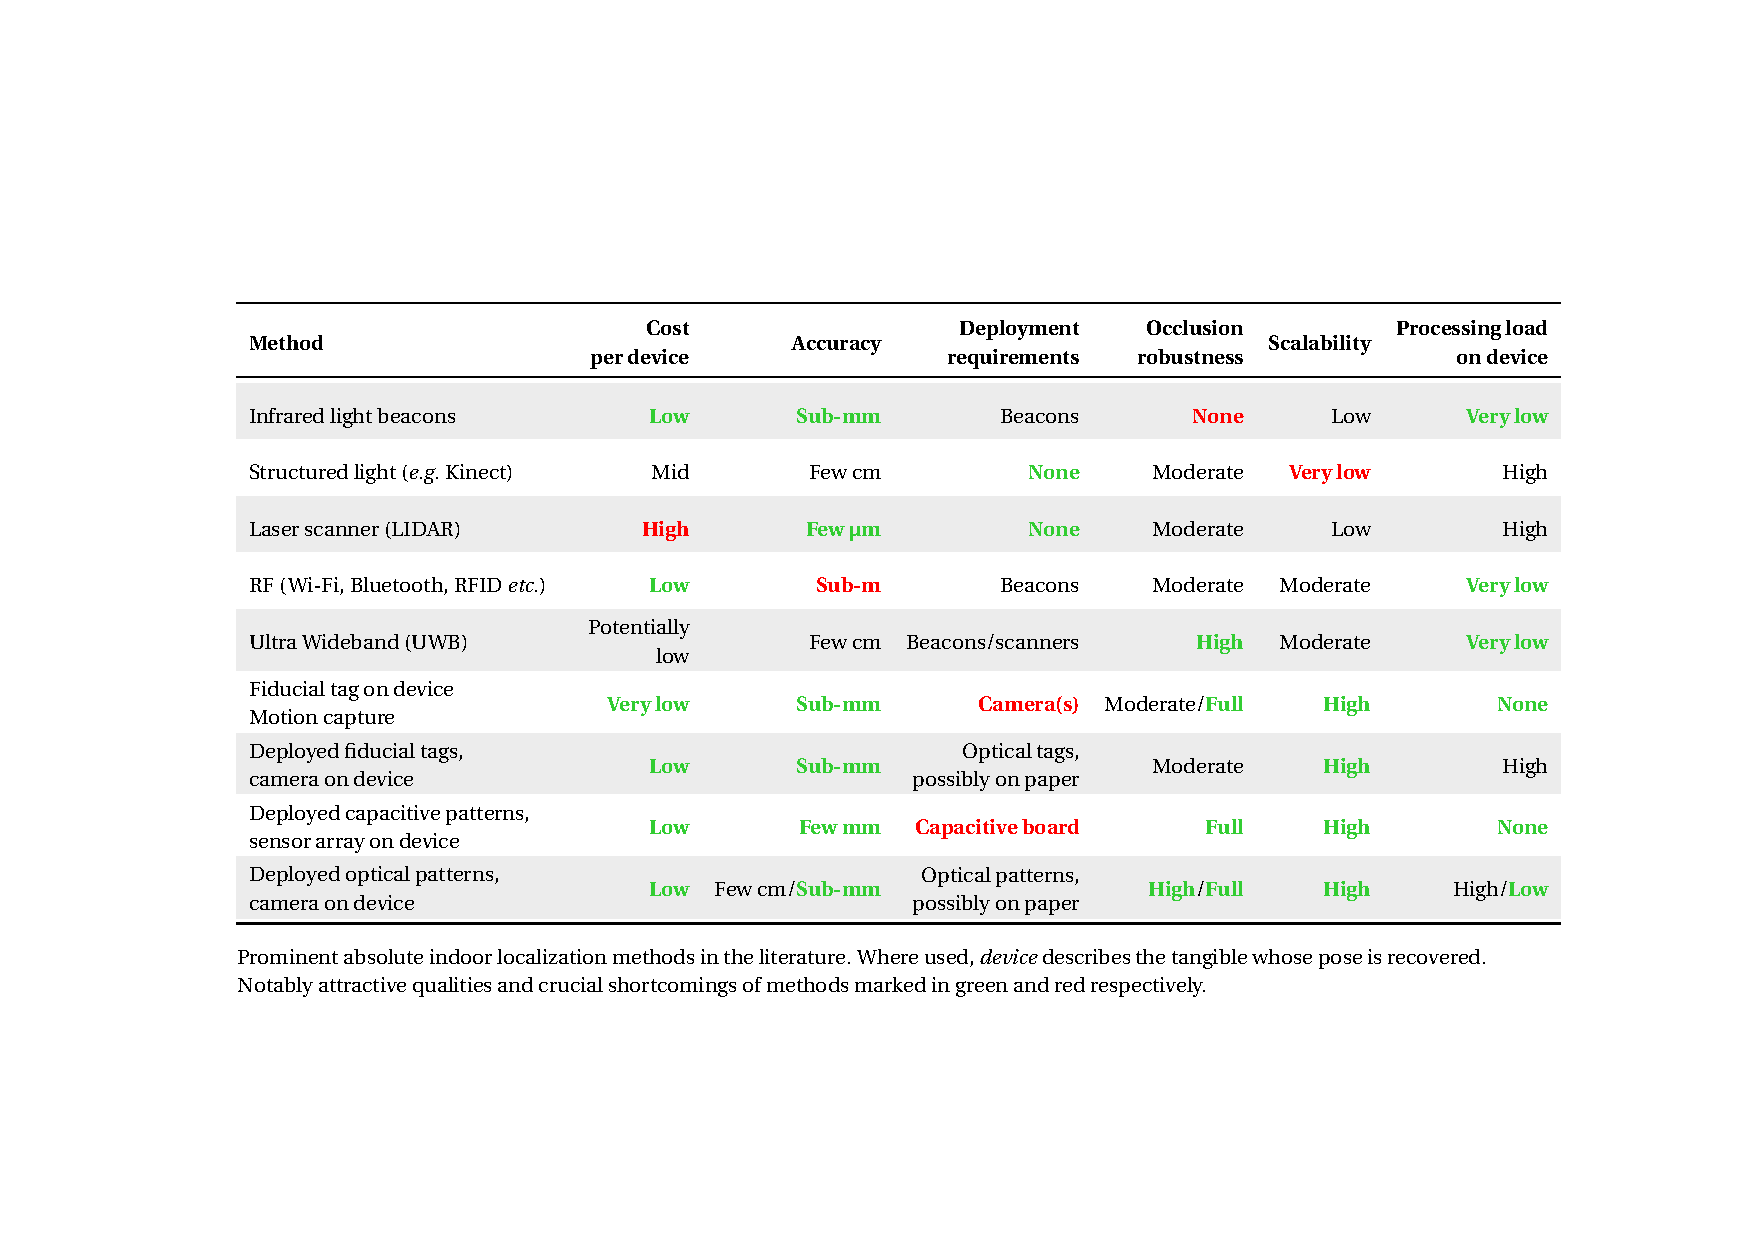
\includepdf{Prominent-absolute-indoor-localization-methods-comparison.pdf} 

% % Please add the following required packages to your document preamble:
% % \usepackage[table,xcdraw]{xcolor}
% % If you use beamer only pass "xcolor=table" option, i.e. \documentclass[xcolor=table]{beamer}
% % \usepackage{lscape}
% \begin{landscape}
%     \begin{table}[htbp]
%     \centering
%     \begin{tabular}{lllllll}
%     \hline
%     Method                                                                                         & Cost per device & Accuracy      & \begin{tabular}[c]{@{}l@{}}Deployment\\ requirements\end{tabular}             & \begin{tabular}[c]{@{}l@{}}Occlusion\\ robustness\end{tabular} & Scalabiity & \begin{tabular}[c]{@{}l@{}}Processing load\\ on device\end{tabular} \\ \hline
%     \rowcolor[HTML]{EFEFEF} 
%     Infrared light beacons                                                                         & Low             & Sub-mm        & Beacons                                                                       & None                                                           & Low        & Very low                                                            \\
%     Structured light (e.g. Kinect)                                                                 & Mid             & Few cm        & None                                                                          & Moderate                                                       & Very low   & High                                                                \\
%     \rowcolor[HTML]{EFEFEF} 
%     Laser scanner (LIDAR)                                                                          & High            & Few µm        & None                                                                          & Moderate                                                       & Low        & High                                                                \\
%     \begin{tabular}[c]{@{}l@{}}RF (Wi-Fi, \\ Bluetooth, RFID etc.)\end{tabular}                    & Low             & Sub-m         & Beacons                                                                       & Moderate                                                       & Moderate   & Very low                                                            \\
%     \rowcolor[HTML]{EFEFEF} 
%     \begin{tabular}[c]{@{}l@{}}Ultra Wideband \\ (UWB)\end{tabular}                                & Potentially low & Few cm        & Beacons/scanners                                                              & High                                                           & Moderate   & Very low                                                            \\
%     \begin{tabular}[c]{@{}l@{}}Fiducial tag on device\\ Motion capture\end{tabular}                & Very low        & Sub-mm        & Camera(s)                                                                     & Moderate/Full                                                  & High       & None                                                                \\
%     \rowcolor[HTML]{EFEFEF} 
%     \begin{tabular}[c]{@{}l@{}}Deployed fiducial tags,\\ camera on device\end{tabular}             & Low             & Sub-mm        & \begin{tabular}[c]{@{}l@{}}Optical tags, \\ possibly on paper\end{tabular}    & Moderate                                                       & High       & High                                                                \\
%     \begin{tabular}[c]{@{}l@{}}Deployed capacitive patterns,\\ sensor array on device\end{tabular} & Low             & Few mm        & Capacitive board                                                              & Full                                                           & High       & None                                                                \\
%     \rowcolor[HTML]{EFEFEF} 
%     \begin{tabular}[c]{@{}l@{}}Deployed optical patterns,\\ camera on device\end{tabular}          & Low             & Few cm/Sub-mm & \begin{tabular}[c]{@{}l@{}}Optical patterns,\\ possibly on paper\end{tabular} & High/Full                                                      & High       & High/Low                                                            \\ \hline
%     \end{tabular}
%     \caption{Prominent absolute indoor localization methods in the literature. Where used, device describes the tangible whose pose is recovered. }
%     \label{tab:localization}
%     \end{table}
% \end{landscape}

% 各类定位方法优缺点\cite{ozgur2018cellulo}如表~\ref{tab:localization}所示。

一类可能有效的定位方式来源于Lee\cite{lee2005moveable}的投影仪辅助定位。


\section{底盘}
考虑到交互过程中需要推动小车,通过用户调查我们知道:大多数用户(特别是儿童)习惯于按压着移动小车,这就使得我们不能采用Zooids\cite{le2016zooids}(如图~\ref{fig:Zooids})或e-puck\cite{mondada2009puck}(如图~\ref{fig:e-puck})使用的差速转向,只能采用类似Cellulo\cite{ozgur2017cellulo}(如图~\ref{fig:Cellulo})的磁驱技术或WolfBot\cite{betthauser2014wolfbot}(如图~\ref{fig:WolfBot})使用的全向轮。

\begin{figure}[htbp]
    \centering
    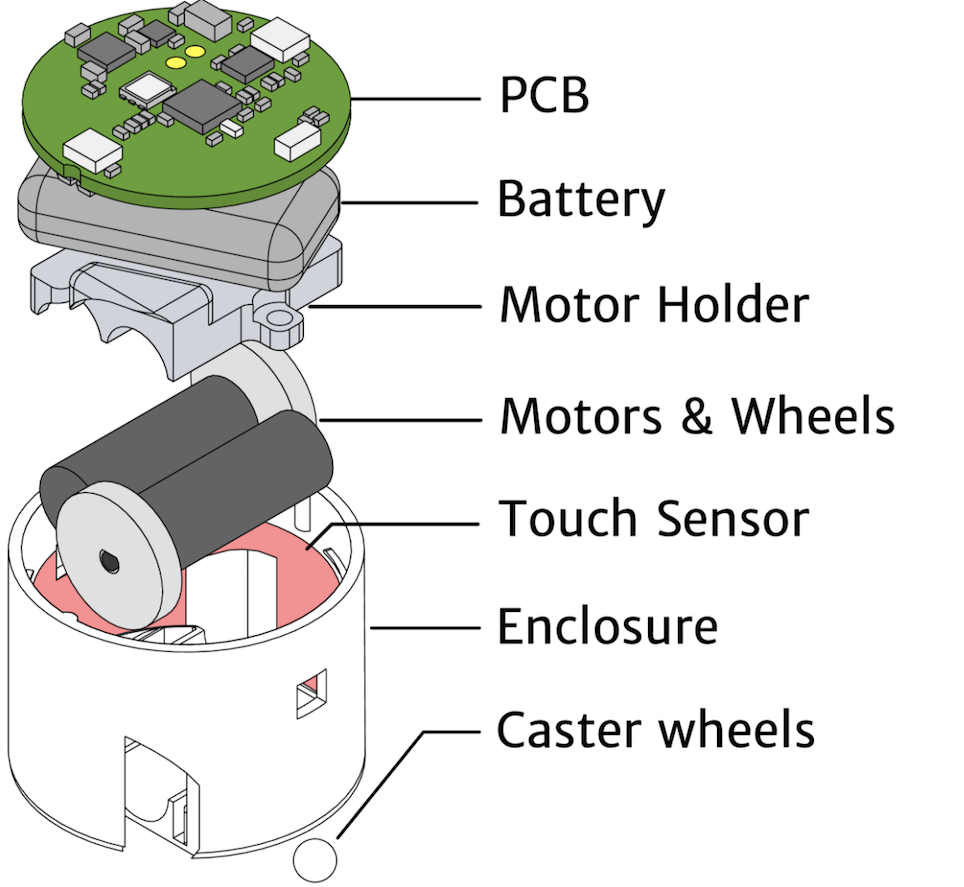
\includegraphics[height=10cm]{Zooids.png}
    \caption{Zooids}
    \label{fig:Zooids}
\end{figure}

\begin{figure}[htbp]
    \centering
    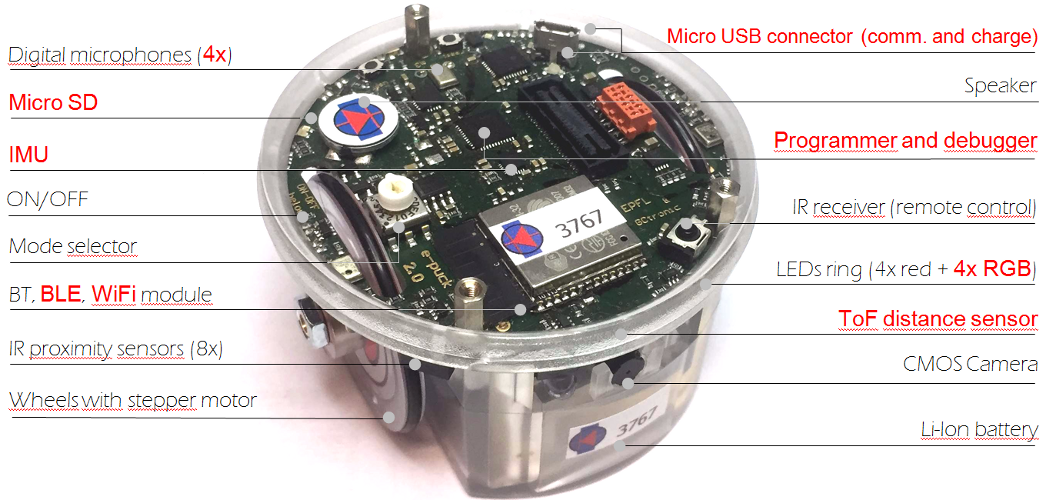
\includegraphics[height=6cm]{e-puck2-features_small.png}
    \caption{Zooids}
    \label{fig:e-puck}
\end{figure}

\begin{figure}[htbp]
    \centering
    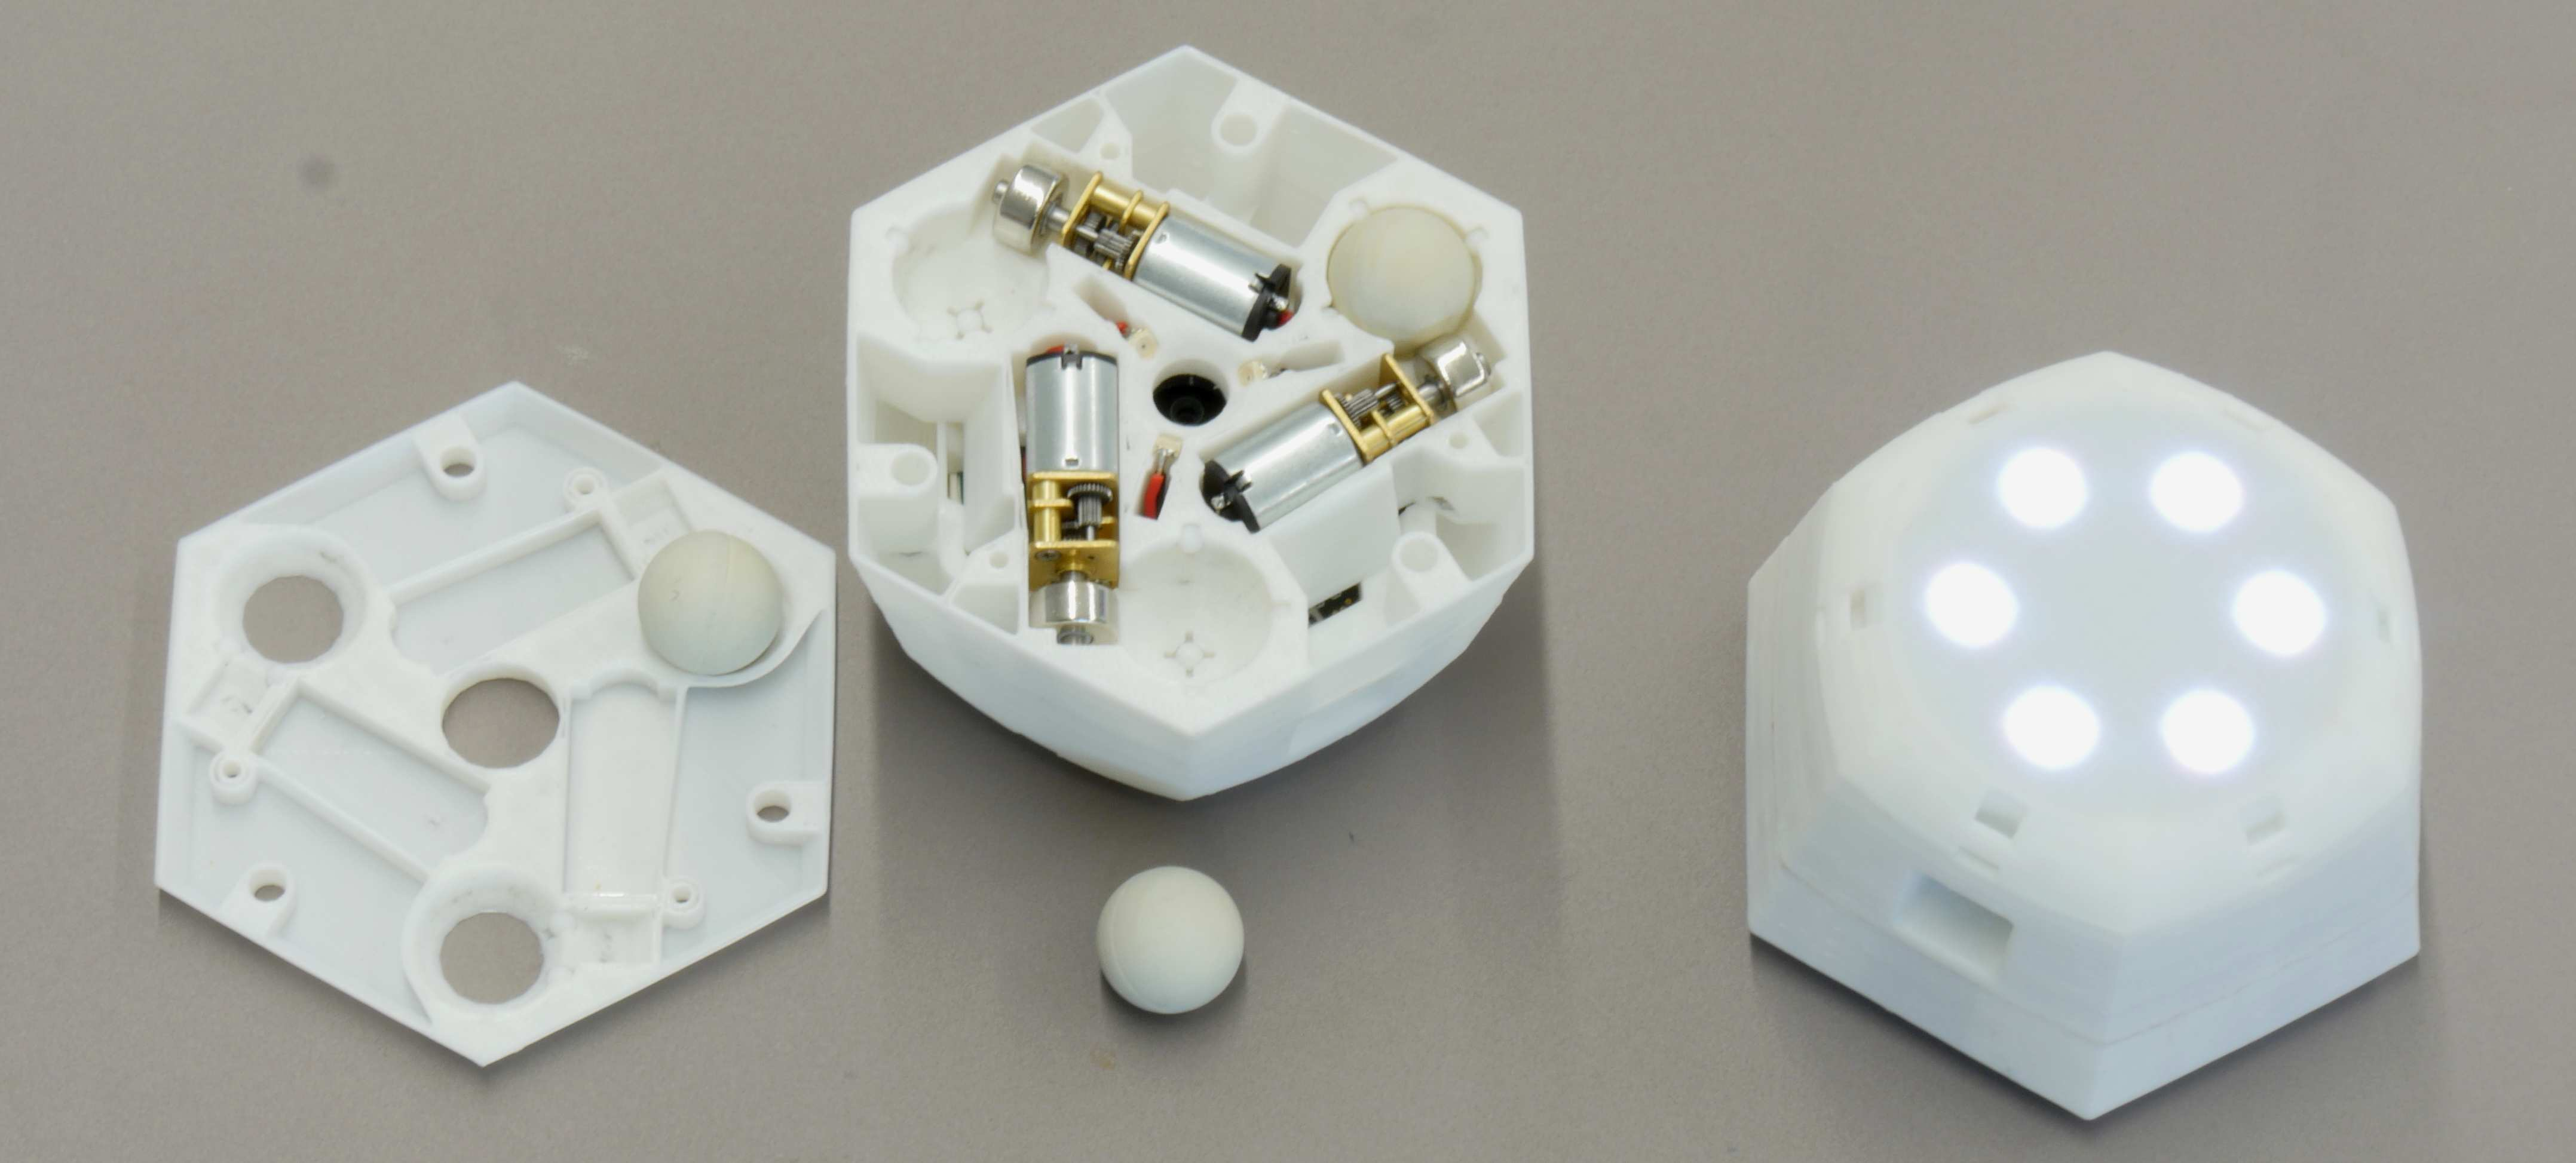
\includegraphics[height=6cm]{cellulo.jpg}
    \caption{Cellulo}
    \label{fig:Cellulo}
\end{figure}
  
\begin{figure}[htbp]
    \centering
    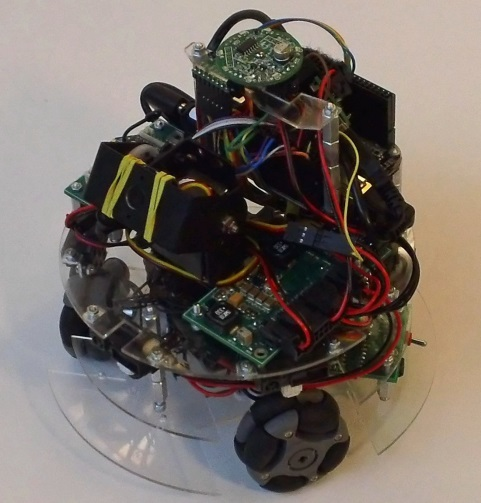
\includegraphics[height=10cm]{WolfBot.jpg}
    \caption{WolfBot}
    \label{fig:WolfBot}
\end{figure}

经过尝试,我们发现磁驱电机的速度和磁环的磁性强弱、电池的电量剩余、磁环和轴之间的胶合强度等不可控因素关系很大,无法建立起小车各轮速度和电机PWM占空比之间的时不变映射关系,导致很难控制小车的走向和速度,最终放弃了这一想法。

WolfBot采用的全向轮和电机直接连接,使得底盘占地面积很大。最终我们则采用1.5英寸麦克纳姆轮(如图~\ref{fig:Wheel})和GW12-N20减速电机(如图~\ref{fig:GM12})(减速齿轮中的蜗杆改变90度传动方向)实现系统最小化。

\begin{figure}
    \begin{minipage}{0.48\textwidth}
      \centering
      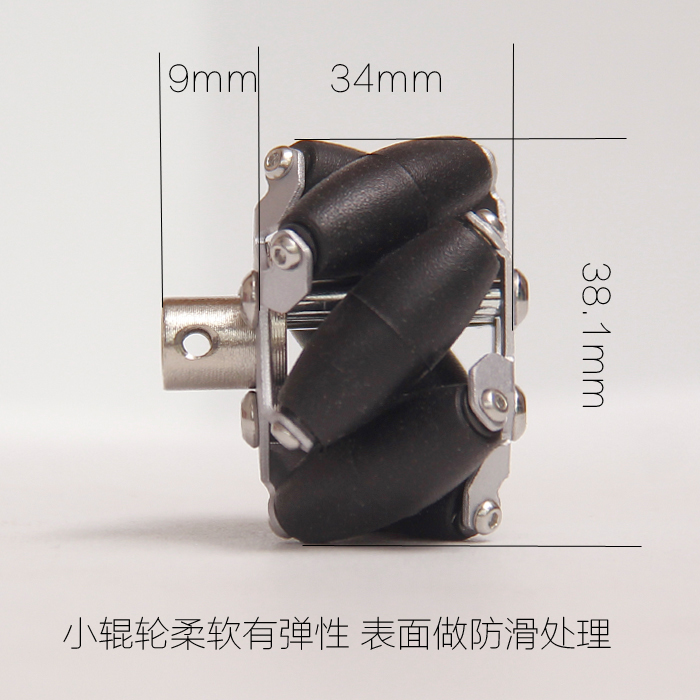
\includegraphics[height=5cm]{Wheel.jpg}
      \caption{使用的1.5英寸麦克纳姆轮}
      \label{fig:Wheel}
    \end{minipage}\hfill
    \begin{minipage}{0.48\textwidth}
      \centering
      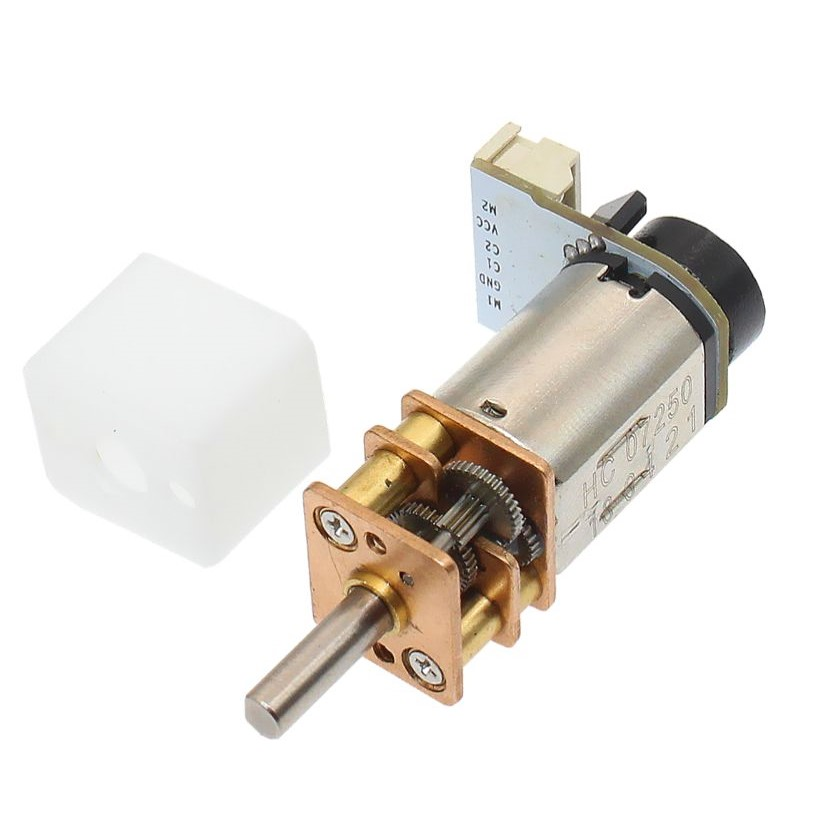
\includegraphics[height=5cm]{CHF-GM12-N20V.jpg}
      \caption{GW12-N20减速电机}
      \label{fig:GM12}
    \end{minipage}
\end{figure}


\section{本项目平台选型}

由于在未来的集群中,单位小车的体积对于总平台需要的面积影响狠大,本项目平台选型首要考量是在功能完备的前提下尽可能缩小平台的体积,特别是直径,同时适度考虑成本。

\subsection{全向轮}

1.5 inch 38mm 90°塑料全向轮(omni wheel)14184 (\url{https://item.taobao.com/item.htm?id=43211511556}) 是目前能找到的直径最小的全向轮,净重约20g。配套的连轴器(Universal hubs)有3MM及4MM六角铜柱,用来连接电机的D形轴。

\subsection{电机}

电机需要提供足够的扭矩,驱动全向轮转动,由于三轮全向轮平台对于各轮转速精确性要求很高,电机需要有反馈,以便进行PID控制,及时调整各电机工作状态。

综上,目前符合要求的电机有两类:一类是微型步进减速电机,步进电机驱动器可以较为精确地控制步进电机的角度值。永磁减速电机加装磁性霍尔或光电编码盘后,码盘可以反馈目前电机的转动方向和转速。

电机有两种备选方案:

\begin{figure}[htbp]
    \centering
    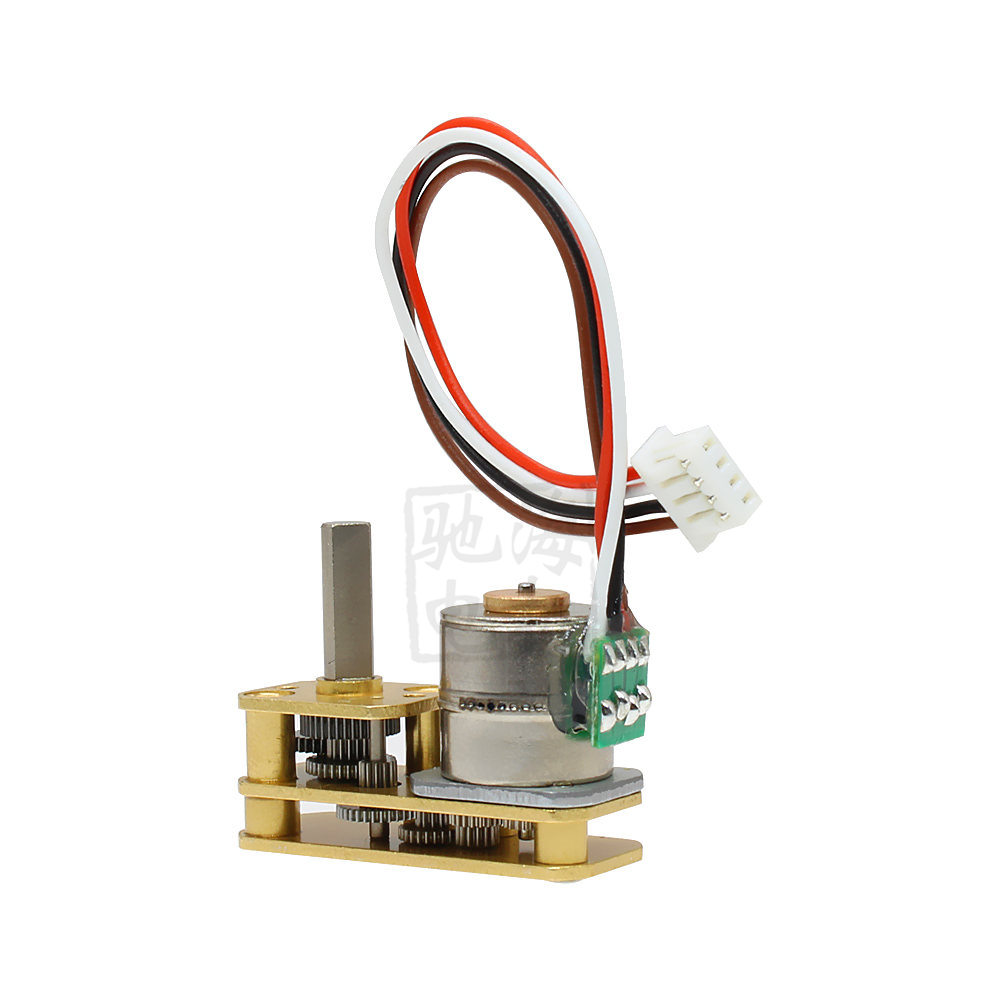
\includegraphics[width=0.46\columnwidth]{CHS-GM12-10BY.jpg}
    \caption{CHS-GM12-10BY}
    \label{fig:CHS-GM12-10BY}
\end{figure}

% 一是使用驰海电机CHS-GM12-10BY 微型步进减速电机 2相4线 电机与轴同向倒装结构 DC5V , 需要定制改变引线方向,现在默认的引线会蹭到轮子,如图~\ref{fig:CHS-GM12-10BY}所示。

一是使用微型步进减速电机, 需要定制改变引线方向,现在默认的引线会蹭到轮子,如图~\ref{fig:CHS-GM12-10BY}所示。

由于微型步进减速电机反折之后比较短小,约为20mm(含出轴和接线端子),可以塞到三个轮子中间。

\begin{figure}[htbp]
    \centering
    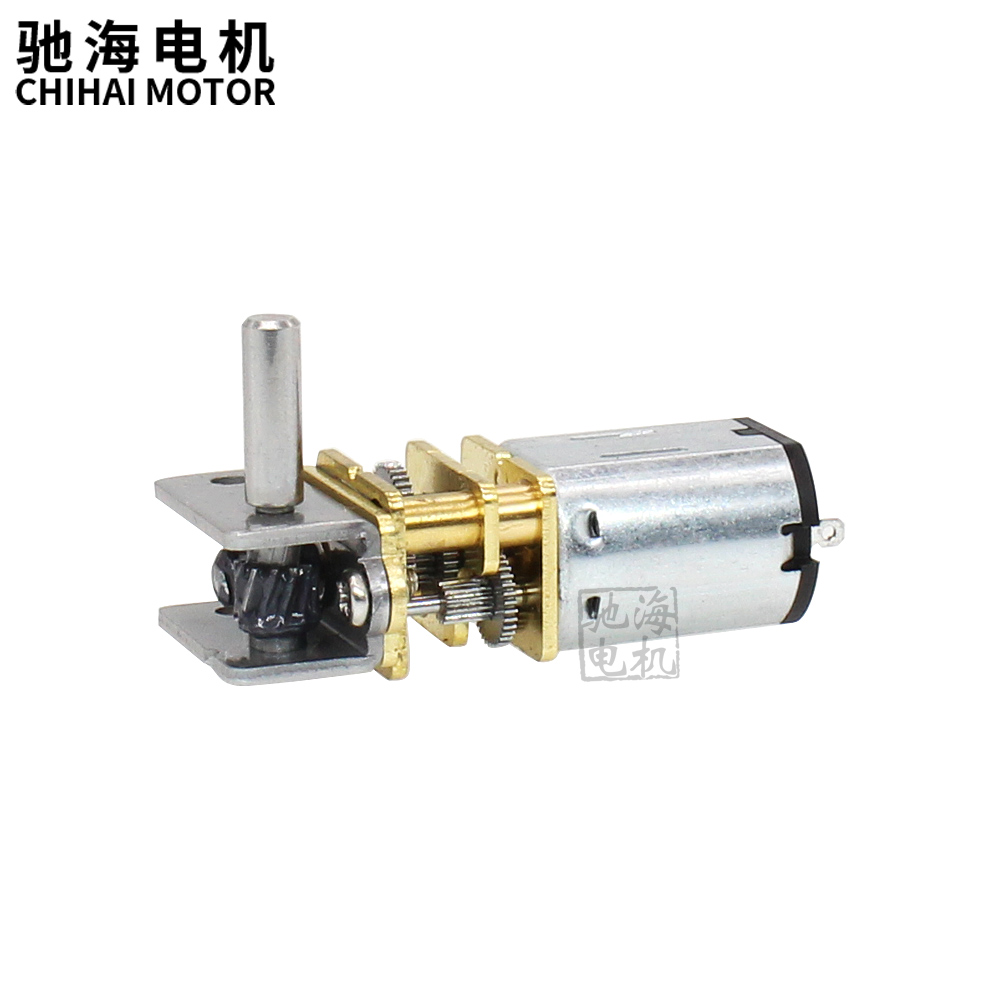
\includegraphics[width=0.46\columnwidth]{CHW-GW12-N20VA.jpg}
    \caption{CHW-GW12-N20VA}
    \label{fig:CHW-GW12-N20VA}
\end{figure}

CHW-GW12-N20VA永磁蜗轮蜗杆齿轮减速电机(有蜗杆改变90度传动方向),定制加装磁性霍尔编码盘,驱动电压5V,空载转速控制在60rpm,如图~\ref{fig:CHW-GW12-N20VA}所示。

蜗杆齿轮减速电机可以垂直装配,占用高度约为40mm。